% =============================================================
% THE BALTIC GROWTH PUZZLE: THREE ECONOMIES UNDER THREE REGIMES
% =============================================================
\section{The Baltic growth puzzle: three economies under three regimes}
\label{sec:baltic}

With the Latvian series in place, the three Baltic economies can be compared with each other and with the rest of Europe on a common footing for the first time. The comparison is organised around the three regimes under which they have lived since 1918, interwar capitalism, Soviet socialism and restored independence, and around the question that the catch-up literature asks of each: did economies that started poor grow faster than the leaders, and if not, why not? Gerschenkron's late industrialiser borrows technology rather than inventing it and substitutes banks or the state for the prerequisites it lacks, and Solow's model predicts faster growth where capital per worker is scarce; Lewis's surplus labour raises average productivity as it moves off the land; and the cumulative effect of all three widens markets and permits scale economies \parencites[8]{gerschenkron1962}[70--1]{solow1956}{lewis1954}[22]{abramovitz_david1996}. But Abramovitz and David argued that the potential is realised only where the follower has the `social capability', the literacy, institutions, managerial competence and commercial organisation, to absorb what it borrows, and where the leader's technology is congruent with the follower's endowments; and Crafts and Toniolo, reading Europe's post-war golden age through that lens, found that even the apparently automatic catch-up of the 1950s and 1960s was conditioned on institutions and policies that fostered investment, technology transfer and the reallocation of resources \parencites[23--35]{abramovitz_david1996}[297--330]{craftstoniolo2010}. The Baltic states are an unusually clean test of these propositions. The human-capital component of their social capability, literacy and schooling, was high throughout, by the standards of the European periphery; its institutional component, the commercial, financial and managerial organisation of the economy, was destroyed and rebuilt twice from outside; and in 1913 all three were among the better-placed peripheral economies of the continent. Tables~\ref{tab:growth} and~\ref{tab:relative} and Figures~\ref{fig:levels} and~\ref{fig:relative} summarise the century.

% tab:growth
\begin{table}[htbp]
\centering\scriptsize\setlength{\tabcolsep}{2.5pt}
\caption{Average annual growth of GDP per capita by regime and sub-period, 1913--2023 (per cent)}
\label{tab:growth}
\begin{threeparttable}
\begin{tabular}{lrrrrrrrrrr}
\toprule
Period & Latvia & Lithuania & Estonia & Baltics & Finland & Nordics & Western & Western & ECE & USSR \\
& & & & & & & core & periphery & & \\
\midrule
\multicolumn{11}{l}{\textit{Interwar capitalism}} \\
\textit{1913--38} & 1.1 & 0.9 & 1.1 & 1.0 & 2.1 & 1.9 & 1.0 & 1.2 & 0.8 & 1.7 \\
\textit{1913--29} & 0.0 & $-$0.2 & 0.2 & 0.0 & 1.6 & 1.8 & 1.0 & 1.4 & 1.3 & $-$0.1 \\
\textit{1929--38} & 3.1 & 3.0 & 2.7 & 2.9 & 3.1 & 2.1 & 1.1 & 0.8 & 0.1 & 5.0 \\
\midrule
\multicolumn{11}{l}{\textit{Soviet socialism (Latvia, Lithuania and Estonia)}} \\
\textit{1938--89} & 2.1 & 2.7 & 2.4 & 2.4 & 3.1 & 2.6 & 2.4 & 3.0 & 2.3 & 2.4 \\
\textit{1938--50} & 1.5 & 0.9 & 2.6 & 1.5 & 1.4 & 2.1 & 0.6 & $-$0.1 & 0.8 & 2.4 \\
\textit{1950--68} & 4.0 & 4.9 & 3.9 & 4.3 & 3.6 & 3.1 & 3.6 & 5.2 & 3.9 & 3.4 \\
\textit{1968--89} & 0.7 & 1.8 & 0.9 & 1.2 & 3.6 & 2.5 & 2.4 & 3.0 & 1.7 & 1.5 \\
\midrule
\multicolumn{11}{l}{\textit{Restored independence}} \\
\textit{1989--2023} & 2.1 & 2.7 & 2.0 & 2.3 & 1.2 & 2.0 & 1.4 & 1.5 & 3.2 & 1.7 \\
\textit{1989--95} & $-$8.9 & $-$6.6 & $-$5.8 & $-$7.2 & $-$0.8 & 1.6 & 1.3 & 2.1 & $-$1.6 & $-$8.0 \\
\textit{1995--2007} & 8.5 & 7.7 & 7.7 & 8.0 & 3.7 & 3.8 & 2.4 & 2.9 & 5.7 & 6.8 \\
\textit{2007--23} & 1.8 & 2.6 & 0.9 & 2.0 & 0.0 & 0.7 & 0.6 & 0.2 & 3.2 & 1.8 \\
\midrule
\textit{1913--2023} & 1.8 & 2.3 & 2.0 & 2.1 & 2.3 & 2.3 & 1.8 & 2.1 & 2.2 & 2.0 \\
\bottomrule
\end{tabular}
\begin{tablenotes}[para,flushleft]
\footnotesize
\textit{Notes:} compound annual rates between end-point years, \intlnineteen{}. Regional rates are growth rates of population-weighted average GDP per capita. Baltics: Latvia, Lithuania and Estonia; Nordics: Denmark, Finland, Iceland, Norway and Sweden; Western core: Austria, Belgium, Denmark, France, Germany (West Germany 1950--97), the Netherlands, Norway, Sweden, Switzerland and the UK; Western periphery: Finland, Greece, Iceland, Ireland, Italy, Portugal and Spain; ECE (East-Central Europe): Bulgaria, Czechoslovakia, Hungary, Poland, Romania and Yugoslavia; USSR: Soviet Union within 1990 borders, former Soviet Union after 1991. \textit{Sources:} Baltic states: this paper, \textcite{klimantas2026soviet} and \textcite{klimantas2025estonia}; other series: \textcite{mpd2023}, extended to 2023 with \textcite{wdi2024} as documented in the online appendix.
\end{tablenotes}
\end{threeparttable}
\end{table}


% tab:relative
\begin{table}[htbp]
\centering\scriptsize\setlength{\tabcolsep}{2.5pt}
\caption{GDP per capita relative to the Western core, the Nordic countries and the USSR, selected years (per cent)}
\label{tab:relative}
\begin{threeparttable}
\begin{tabular}{lrrrrrrrrrr}
\toprule
& \multicolumn{6}{c}{Percentage of Western core} & \multicolumn{3}{c}{Percentage of Nordics} & USSR \\
\cmidrule(lr){2-7}\cmidrule(lr){8-10}\cmidrule(lr){11-11}
Year & Latvia & Lithuania & Estonia & Baltics & W.\ periphery & ECE & Latvia & Lithuania & Estonia & Latvia \\
\midrule
1913 & 59 & 41 & 51 & 49 & 55 & 39 & 80 & 56 & 70 & --- \\
1929 & 50 & 34 & 45 & 42 & 58 & 41 & 59 & 40 & 53 & --- \\
1938 & 60 & 40 & 52 & 49 & 57 & 37 & 65 & 43 & 56 & 144 \\
\midrule
1950 & 67 & 41 & 66 & 55 & 52 & 38 & 61 & 37 & 60 & 144 \\
1968 & 72 & 51 & 70 & 62 & 69 & 40 & 71 & 50 & 69 & 159 \\
1973 & 67 & 51 & 63 & 59 & 71 & 40 & 66 & 50 & 62 & 155 \\
1989 & 51 & 45 & 52 & 48 & 78 & 35 & 50 & 45 & 51 & 136 \\
\midrule
1995 & 27 & 28 & 33 & 28 & 82 & 29 & 28 & 29 & 34 & --- \\
2008 & 52 & 52 & 58 & 53 & 85 & 45 & 49 & 49 & 55 & --- \\
2019 & 59 & 66 & 65 & 63 & 79 & 57 & 58 & 65 & 64 & --- \\
2023 & 64 & 69 & 65 & 67 & 81 & 63 & 61 & 66 & 61 & --- \\
\bottomrule
\end{tabular}
\begin{tablenotes}[para,flushleft]
\footnotesize
\textit{Notes:} \intlnineteen{}; regional aggregates are population-weighted. The last column gives Latvian GDP per capita as a percentage of the Soviet average within 1990 borders; from 1946 the Soviet level is Maddison's series rescaled to Bolotin's 1990 benchmark, to which the Latvian series is anchored (1938 uses Maddison's level and is the less certain). Country groups as in Table~\ref{tab:growth}. \textit{Sources:} as Table~\ref{tab:growth}.
\end{tablenotes}
\end{threeparttable}
\end{table}


\begin{figure}[htbp]
\centering
\caption{GDP per capita in the Baltic states, Finland, the Western core and the USSR, 1913--2023}
\label{fig:levels}
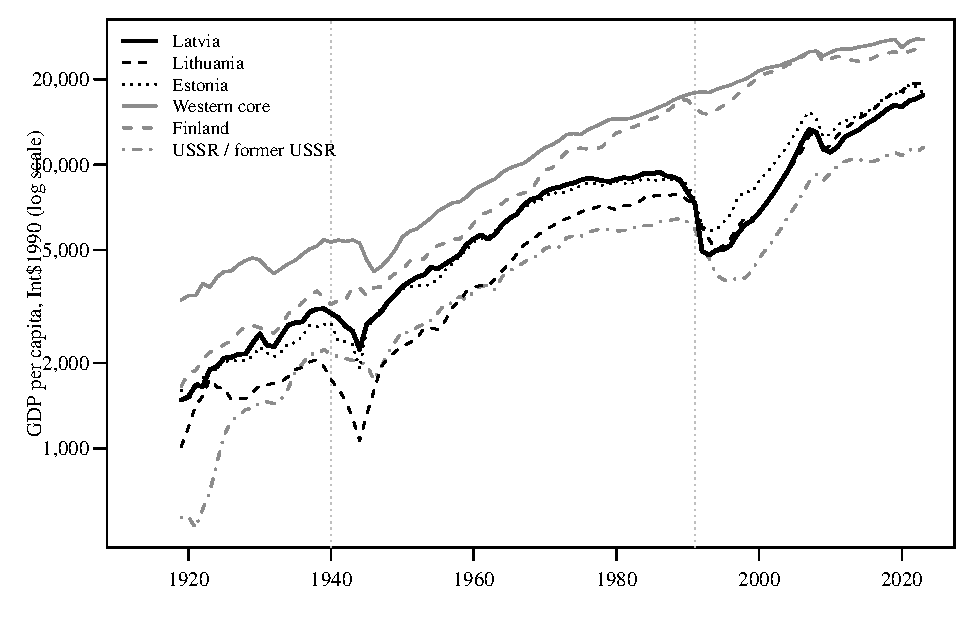
\includegraphics[width=\textwidth]{F1_levels.pdf}
\begin{minipage}{0.95\textwidth}\footnotesize
\textit{Notes:} \intlnineteen{}, log scale; 1914--18 not estimated. Vertical lines mark the Soviet occupation of 1940 and the restoration of independence in 1991. USSR within 1990 borders, former Soviet Union after 1991. \textit{Sources:} as Table~\ref{tab:growth}.
\end{minipage}
\end{figure}

\begin{figure}[htbp]
\centering
\caption{GDP per capita as a percentage of the Western core, 1913--2023, five-year moving averages}
\label{fig:relative}
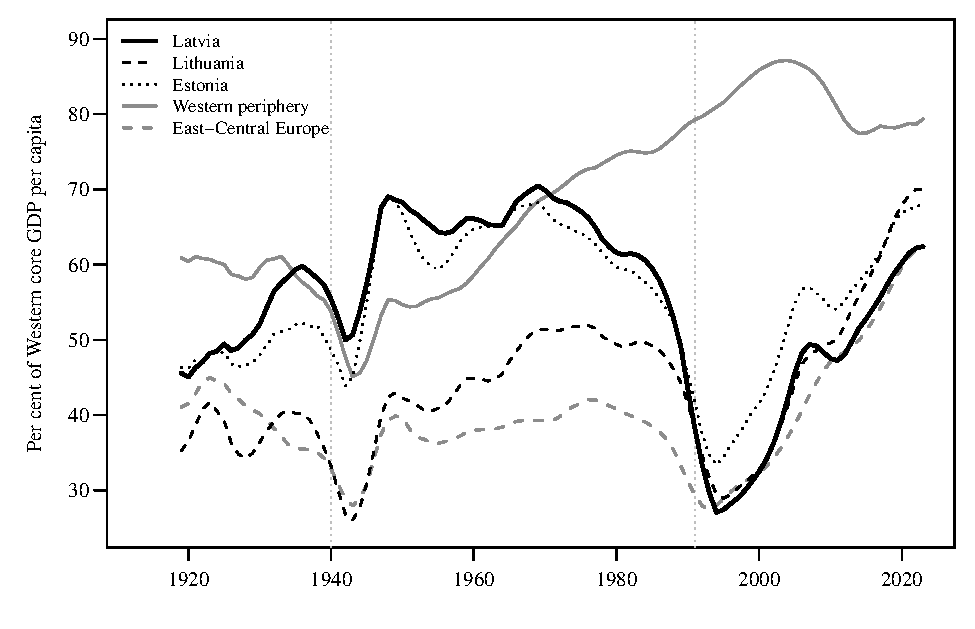
\includegraphics[width=\textwidth]{F2_relative.pdf}
\begin{minipage}{0.95\textwidth}\footnotesize
\textit{Notes:} population-weighted regional aggregates; country groups as in Table~\ref{tab:growth}. \textit{Sources:} as Table~\ref{tab:growth}.
\end{minipage}
\end{figure}

The puzzle that the long series reveal is this. In 1913 Latvia stood at \pctwc{1913} per cent of the income per head of the Western core and Estonia at \pctx{Estonia}{Western}{1913}, levels comparable to Finland's and Italy's; Lithuania, at \pctx{Lithuania}{Western}{1913} per cent, exceeded Greece and Portugal. All three were literate, serfdom had ended in Latvia and Estonia in 1816--19, two generations before Russia, and all three would carry out the most radical land reforms in Europe within a decade. Yet by 2023, after a century in which they grew under three different systems, Latvia stood at \pctwc{2023} per cent of the Western core, Estonia at \pctx{Estonia}{Western}{2023} and Lithuania at \pctx{Lithuania}{Western}{2023}: the region as a whole had moved from \pctx{Baltics}{Western}{1913} to \pctx{Baltics}{Western}{2023} per cent, a gain of eighteen percentage points over 110 years, and against the Nordic countries Latvia had fallen from \pctnord{1913} to \pctnord{2023} per cent. The Western periphery, the group of poorer Western economies to which the Baltic states belonged by income in 1938, rose over the same century from \pctx{Periphery}{Western}{1913} to \pctx{Periphery}{Western}{2023} per cent. Within the region the ranking reversed: Latvia, the richest Baltic economy in 1913, in 1938 and in all but a handful of years to 1988 (Estonia stood marginally above it in the aftermath of each war, 1919--23 and 1947--8, and in 1962--4), is now the poorest, and Lithuania, the poorest for most of the century, is the richest. The sections below take the three regimes in turn.

\subsection{Interwar capitalism, 1913--1940}

The First World War and the collapse of the empires gave Lithuania, Latvia and Estonia their first opportunity to build independent states, and left them in ruins. The German advance of 1915 stabilised along the Daugava, within reach of Riga, for two and a half years; the imperial government evacuated Latvia's industry eastwards, and most of it never returned; Riga lost more than half its population between 1914 and 1919 \parencites[107]{ehbaltics_tarvel}[616]{norkusmark2021}. Table~\ref{tab:war} places the result beside the other belligerents. Between 1913 and 1919 Latvia lost 35 per cent of its population, 59 per cent of its GDP and 37 per cent of its income per head, Lithuania 36, 60 and 38 per cent; of the European economies for which estimates exist, only the Soviet Union lost as large a share of its output. Estonia, untouched by major fighting until 1918, lost less. Pre-war Latvia had been called the `Belgium of the East' for its industry and living standards; by 1919 it resembled Belgium in the devastation it had suffered relative to its size \parencite[77]{hiden_salmon}.

% tab:war
\begin{table}[htbp]
\centering\small
\caption{Demographic and economic impact of the two world wars (percentage change)}
\label{tab:war}
\begin{threeparttable}
\begin{tabular}{lrrr}
\toprule
& Population & GDP & GDP per capita \\
\midrule
\multicolumn{4}{l}{\textit{(a) First World War: decline from 1913 to the 1918/19 trough}} \\
Austria & $-$5 & $-$38 & $-$35 \\
Belgium & 0 & $-$32 & $-$32 \\
France & $-$7 & $-$25 & $-$31 \\
USSR & $-$1 & $-$60 & $-$59 \\
Lithuania & $-$36 & $-$60 & $-$38 \\
Latvia & $-$35 & $-$59 & $-$37 \\
Estonia & $-$9 & $-$29 & $-$22 \\
\midrule
\multicolumn{4}{l}{\textit{(b) Second World War: decline from 1938 to the 1944--6 trough}} \\
Greece & 3 & $-$64 & $-$65 \\
Germany & $-$6 & $-$58 & $-$56 \\
Austria & 1 & $-$51 & $-$52 \\
Netherlands & 6 & $-$47 & $-$50 \\
Poland & $-$23 & $-$57 & $-$49 \\
Lithuania & $-$5 & $-$48 & $-$48 \\
Latvia & $-$23 & $-$40 & $-$28 \\
Estonia & $-$20 & $-$42 & $-$29 \\
\bottomrule
\end{tabular}
\begin{tablenotes}[para,flushleft]
\footnotesize
\textit{Notes:} each column is measured from the pre-war year to its own trough within the window named. Lithuania in panel (b) within actual borders (the 1939 loss of Klaip\.{e}da and gain of Vilnius); within post-war borders its population fell by 22 per cent. \textit{Sources:} Baltic states: this paper and the companion series; others: \textcite{mpd2023}.
\end{tablenotes}
\end{threeparttable}
\end{table}


The 1920s were a decade of reconstruction rather than growth. Lithuania regained its 1913 income per head by 1923, Estonia by 1925, Latvia only in \lvREGAINthirteen{}: the recovery was most protracted where the pre-war economy had been most integrated into the Russian market and most of the industrial capacity had been lost \parencites[95--6]{aldcroftthirdworld}[103]{eastern_crampton}. Between 1913 and 1929 income per head in the three countries together was unchanged (Table~\ref{tab:growth}), while the Western core grew by \grx{Western}{1913}{1929} per cent a year and Czechoslovakia, Berend's `success story of the twenties', by 45 per cent \parencite[243]{Berenddecadesofcrisis}; Latvia's 1922--9 growth of \gr{1922}{1929} per cent a year was bounce-back growth from a very low base, financed by foreign capital, and it stopped when the pre-war level was regained. The new states rebuilt on the land. Agrarian reforms expropriated the estates of the Baltic-German and Polish nobility, which had held between a quarter and a half of all land, and created a class of smallholders; gold-backed currencies were introduced in 1922 (Latvia and Lithuania) and 1928 (Estonia); exports were redirected from Russia to Britain and Germany and shifted from manufactures to butter, bacon, flax and timber, in conscious imitation of Denmark \parencites[115]{baltichistorykasekamp2017}{norkus_2025_denmarkisation}. Agriculture still employed 67 per cent of the Latvian labour force in the late 1930s and 63 and 74 per cent of the Estonian and Lithuanian (Table~\ref{tab:structure}).

The 1930s look different. Between 1929 and 1938 income per head grew by \gr{1929}{1938} per cent a year in Latvia, \grx{Lithuania}{1929}{1938} in Lithuania and \grx{Estonia}{1929}{1938} in Estonia, against \grx{Western}{1929}{1938} per cent in the Western core, \grx{Periphery}{1929}{1938} in the Western periphery and \grx{ECE}{1929}{1938} in East-Central Europe; among European economies only the Soviet Union, whose figures for the period are contested, and Finland grew as fast, and all three Baltic states closed their gap with the Western core by six to ten percentage points (Table~\ref{tab:relative}). The Depression was shallower and shorter than in most of Europe: Lithuania avoided recession altogether, and Latvia's and Estonia's downturns of 1931--3, of 10 and 8 per cent from peak to trough, resembled those of the Nordic countries, which are regarded as among the mildest on the continent \parencite{grytten_nordicdepression}. The Baltic performance has usually been read, by contemporaries and by Aldcroft, as the fruit of export-led agricultural modernisation \parencites[189]{balticstates1938}[119--20]{aldcrof1914}. The sectoral evidence does not support that reading. Trade openness fell sharply after 1929, in Latvia from 38 to 22 per cent of GDP, the processed share of exports fell in both Latvia and Estonia, and the Baltic states remained the most agrarian and least industrial part of Europe outside the Balkans (Table~\ref{tab:structure}). What grew was industry for the home market: Latvian industrial output rose by \sgr{Industry}{1929}{1938} per cent a year over 1929--38, a rate exceeded among capitalist economies only by Lithuania and matched only by Finland, behind import-substituting tariffs, state enterprises and the infant-industry policies that the authoritarian governments of the 1930s, Lithuania's dating from 1926 and Estonia's and Latvia's from 1934, adopted as part of their `economic nationalism' \parencites[116]{ehbaltics_tarvel}{karnups_2017_karla}{Klimantas2024}. Latvia was the one Baltic economy in which the shares of both agriculture and industry in GDP rose in the 1930s at the expense of services, the result of heavily subsidised agriculture and the pruning of the public administration \parencite[683]{latvija19141945vesture}. The growth of the 1930s was achieved not through international trade but despite its contraction.

% tab:structure
\begin{table}[htbp]
\centering\scriptsize\setlength{\tabcolsep}{2pt}
\caption{Economic structure, industrial growth and openness: the Baltic states and their peers, c.\,1937 and c.\,1990}
\label{tab:structure}
\begin{threeparttable}
\resizebox{\textwidth}{!}{\begin{tabular}{lrrrrrrrrrr}
\toprule
& \multicolumn{3}{c}{Share of GDP, c.\,1937} & \multicolumn{3}{c}{Share of GDP, c.\,1990} & Agr.\ empl. & Ind.\ growth & \multicolumn{2}{c}{Trade openness} \\
\cmidrule(lr){2-4}\cmidrule(lr){5-7}\cmidrule(lr){8-8}\cmidrule(lr){9-9}\cmidrule(lr){10-11}
& Agr. & Ind. & Serv. & Agr. & Ind. & Serv. & c.\,1938 & 1929--38 & 1925/9 & 1935/8 \\
\midrule
Lithuania & 44 & 18 & 38 & 22 & 36 & 42 & 74 & 8.0 & 20 & 22 \\
Latvia & 40 & 23 & 37 & 18 & 35 & 47 & 67 & 6.8 & 38 & 22 \\
Estonia & 38 & 23 & 40 & 17 & 41 & 42 & 63 & 5.7 & 35 & 31 \\
Baltics & 40 & 21 & 38 & 19 & 37 & 44 & 68 & 6.9 & --- & --- \\
\midrule
Finland & 32 & 30 & 38 & 7 & 34 & 60 & 57 & 6.3 & 42 & 34 \\
Iceland & 44 & 16 & 40 & 10 & 25 & 65 & 46 & 3.7 & 88 & 49 \\
Ireland & 25 & 24 & 51 & 12 & 46 & 43 & 48 & 4.6 & 79 & 50 \\
USSR & 31 & 32 & 37 & 19 & 41 & 40 & 65 & 10.3 & --- & --- \\
Czechoslovakia & 24 & 35 & 41 & 17 & 48 & 35 & 37 & $-$0.8 & --- & --- \\
Hungary & 34 & 30 & 37 & 24 & 38 & 38 & 53 & 3.6 & --- & --- \\
Bulgaria & 52 & 15 & 33 & 13 & 57 & 30 & 80 & 3.0 & --- & --- \\
Portugal & 30 & 27 & 43 & 7 & 38 & 55 & 49 & 2.2 & 22 & 20 \\
Greece & 54 & 26 & 20 & 14 & 25 & 61 & --- & 5.7 & 22 & 16 \\
\midrule
Western core & 14 & 38 & 49 & 3 & 32 & 65 & 25 & 1.1 & --- & --- \\
Western periphery & 36 & 26 & 39 & 8 & 35 & 56 & 50 & 3.3 & --- & --- \\
East-Central Europe & 37 & 27 & 36 & 14 & 36 & 46 & 65 & 2.2 & --- & --- \\
\bottomrule
\end{tabular}}
\begin{tablenotes}[para,flushleft]
\footnotesize
\textit{Notes:} shares of gross value-added at current prices; `Ind.' includes construction. c.\,1937 is the average of 1935--9 and c.\,1990 of 1985--93 where annual data exist, otherwise the nearest year (1990 for the Baltic states and ECE). Regional shares are simple averages. Agricultural employment share and industrial output growth (compound annual rate) from the comparator datasheets of the online appendix, which give the source of each cell; trade openness is exports plus imports as a percentage of GDP, averaged over the years shown; `---' not available. \textit{Sources:} GDP shares: this paper (benchmarks of Table~\ref{tab:benchmarks}), \textcite{klimantas2019}, \textcite{klimantas2025estonia}, \textcite[179]{morysinterwarinmorys2021}, \textcite{mitchelstat}, \textcite[158]{portugal_economy}, \textcite[24]{jonsson1999}, \textcite[460]{ivanov2012gdp}, \textcite[184]{bolotin1992}, \textcite[182]{un_yearbook1993}, \textcite[346]{cameh_sectoral1945}; employment and industrial growth: \textcite[181]{morysinterwarinmorys2021}, \textcite{mitchelstat}, \textcite[2]{ostlandinzahlen}, \textcite[86]{east_industry_periphery1871}; trade: \textcite{lidaexportslv,lidaimportslv}, \textcite{worldtrade1949}, \textcite[123, 161]{balticstates1938}, \textcite[21]{jonsson1999}.
\end{tablenotes}
\end{threeparttable}
\end{table}


The verdict on the interwar regime is mixed. Over 1913--38 as a whole, Latvian and Estonian income per head grew marginally faster than the Western core's, by \gr{1913}{1938} and \grx{Estonia}{1913}{1938} against \grx{Western}{1913}{1938} per cent a year, and Lithuanian marginally slower; the region's position relative to the core, \pctx{Baltics}{Western}{1913} per cent in 1913 and \pctx{Baltics}{Western}{1938} in 1938, did not change. The 1930s were among the most dynamic years the region has known, and by 1938 Latvia and Estonia retained the places among the best-performing peripheral economies of Europe that they had held in 1913, which is what Aldcroft meant in calling the Baltic states the most promising of Europe's backward regions \parencite[105, 171]{aldcroftthirdworld}. But the interwar years also disposed of a belief that has shaped Baltic self-perception ever since: that Latvia and Estonia stood level with Finland. They had been close in 1913, Latvia at \pctfin{1913} per cent of the Finnish level; by 1938 Latvia stood at \pctfin{1938} per cent and Estonia at \pctx{Estonia}{Finland}{1938}, because Finland grew at \grx{Finland}{1913}{1938} per cent a year through the two decades while the Baltic economies spent the first of them recovering what the war had destroyed. The difference was not one of social capability: Latvian literacy was above Finnish and Latvian university enrolment per head, 4.3 per thousand in the 1930s, nearly double the Western core's \parencite{klimantas2025thesis}. It was one of resources and markets. Finland's forests gave it an export staple for which Western demand recovered quickly after 1920 and which carried an engineering sector with it; the Baltic states had lost the only large market their industry had ever served, and the food exports that replaced it faced Danish competition and British quotas.

\subsection{Soviet socialism, 1940--1991}

The Soviet occupation of June 1940, the German occupation of 1941--4 and the renewed fighting of 1944 cost Latvia and Estonia a fifth or more of their population, Lithuania within its actual borders a twentieth, and the three, on the present estimates, between 28 and 48 per cent of their income per head (Table~\ref{tab:war}). The losses were demographic before they were material: deportations, the Holocaust, war deaths and the flight of some 250,000 people to the West in 1944 removed more than a million people, among them a disproportionate share of the professional and commercial classes; the fall in income per head, 28 per cent in Latvia and 29 in Estonia, was correspondingly smaller than the fall in output, and roughly half the per-capita losses that Table~\ref{tab:war} records for Austria, the Netherlands or Poland. Lithuania's larger fall is examined in the companion paper. Recovery was rapid, as it was everywhere in the Soviet sphere: Latvia regained its 1938 level of total GDP in \sregain{GDP}, Estonia its 1939 level in 1948 and Lithuania in 1949, and with smaller populations their income per head regained the 1938 level in 1946, \lvREGAINthirtyeight{} and 1948 respectively, two years before the Western core or periphery regained theirs. The war had destroyed people rather than plant; with a fifth of the population of the northern republics gone, capacity stood underused, and the early recovery rested on putting labour, increasingly immigrant labour directed from Russia, back to work on existing capital, the mechanism that Vonyó and Markevich identify across post-war East-Central Europe \parencites[290]{vonyoinmorys2021}[108]{years_of_dependence}.

The command economy was installed within five years. Industry and banks were nationalised in 1940--1 and again in 1945--7; the republics were incorporated into the all-Union planning system in 1946; and the deportations of 1948--53, which removed some 42,000 people from Latvia, 100,000 from Lithuania and 35,000 from Estonia, the largest single operation being that of March 1949, which took more than 40,000 people from Latvia and some 30,000 and 21,000 from Lithuania and Estonia, broke the resistance of the countryside to collectivisation, which was essentially complete within two years (Table~\ref{tab:collectivisation}). The agricultural indices record the cost. Latvian agricultural output, which had already fallen to 59 per cent of its 1938 level in 1947, hovered between 60 and 67 per cent through 1955, regained the pre-war level only in \sregain{Primary}, twenty-nine years after the pre-war peak, and never exceeded \primPEAKidx{} per cent of it before 1991, despite mechanisation and fertiliser; Estonia's recovery came in 1959 and Lithuania's in 1957. Nothing comparable to the Soviet famine of 1932--3 occurred, probably because the Baltic collectivisation did not coincide with a procurement crisis and because the system had by then learned to extract the surplus without destroying the herds; but in every Baltic republic the private plots that occupied a tenth of the land were producing a quarter to a third of agricultural output in 1989 \parencites{labsvirs_1959_case}[187--91]{years_of_dependence}.

% tab:collectivisation
\begin{table}[htbp]
\centering\footnotesize
\caption{Collectivisation of Baltic agriculture, 1947--55}
\label{tab:collectivisation}
\begin{threeparttable}
\begin{tabular}{lrrrrrr}
\toprule
& \multicolumn{2}{c}{Latvia} & \multicolumn{2}{c}{Lithuania} & \multicolumn{2}{c}{Estonia} \\
\cmidrule(lr){2-3}\cmidrule(lr){4-5}\cmidrule(lr){6-7}
& Farms & Output & Farms & Output & Farms & Output \\
& coll.\ (\%) & 1938 = 100 & coll.\ (\%) & 1938 = 100 & coll.\ (\%) & 1938 = 100 \\
\midrule
1947 & ${<}$1 & 59 & ${<}$1 & 82 & 0 & 81 \\
1948 & 2 & 67 & ${<}$1 & 86 & 0 & 90 \\
1949 & 10 & 64 & 4 & 94 & 6 & 86 \\
1950 & 85 & 67 & 62 & 91 & 80 & 85 \\
1951 & 97 & 64 & 89 & 82 & 93 & 83 \\
1952 & 98 & 65 & ${>}$90 & 76 & 97 & 84 \\
1953 & ${>}$98 & 61 & 94 & 77 & 99 & 80 \\
1954 & ${>}$98 & 64 & ${>}$94 & 83 & ${>}$99 & 79 \\
1955 & ${>}$98 & 60 & ${>}$94 & 78 & ${>}$99 & 77 \\
\midrule
Deported, 1940--53 & \multicolumn{2}{c}{58,000 (3\%)} & \multicolumn{2}{c}{132,000 (5\%)} & \multicolumn{2}{c}{45,000 (4\%)} \\
\quad of which 1948--53 & \multicolumn{2}{c}{42,000} & \multicolumn{2}{c}{100,000} & \multicolumn{2}{c}{35,000} \\
\bottomrule
\end{tabular}
\begin{tablenotes}[para,flushleft]
\footnotesize
\textit{Notes:} `Farms coll.': share of farms collectivised at the beginning of the year (mid-year for Estonia in 1952--3); output is the volume index of agricultural value-added (crops and livestock). Deportations in brackets as a share of the population. \textit{Sources:} output: this paper and companion series; collectivisation and deportations: \textcite[69]{lv_collectiv}; \textcite[241--2]{lv_sovhist02}; \textcite{lv_deportations}; \textcite[471]{Girnius1988}; \textcite{vlekolektyv}; \textcite[265]{taagepera_coll01}; \textcite[12]{deportations_ee}.
\end{tablenotes}
\end{threeparttable}
\end{table}


What collectivisation did deliver was labour. Industry and construction expanded in the 1950s at rates the capitalist republics had never seen: Latvian industrial output grew by \sgr{Industry}{1950}{1968} per cent a year over 1950--68 and construction by \sgr{Construction}{1950}{1968}, Lithuanian industry by 10 per cent a year to 1975. The mechanism was the Soviet one of the 1930s, the forced migration of labour from countryside to town and the extraction of the agricultural surplus for reinvestment \parencite[99, 190, 211]{allenfarm}. Lithuania, where 80 per cent of the population still lived on the land in 1946, had the labour reserve to sustain it; Latvia and Estonia, more urban and with low fertility, did not, and the planners drew instead on immigration from the Russian interior, which raised Latvia's population by \lvPOPchangeSOVIET{} per cent between 1950 and 1989 and reduced ethnic Latvians to barely half of it \parencite[126--8]{baltichistorykasekamp2017}. Each republic was assigned a role in the Union's division of labour: Lithuania food processing, light industry and, later, oil refining and nuclear power; Estonia oil shale, electricity and textiles; Latvia machine-building, the electrotechnical and radio industry, railway rolling stock and microbuses, and a disproportionate share of all-Union and military enterprises \parencites[203--15]{years_of_dependence}{gatis_lv_eh}. Table~\ref{tab:growth} records the result. Between 1950 and 1968 income per head grew by \gr{1950}{1968} per cent a year in Latvia, \grx{Estonia}{1950}{1968} in Estonia and \grx{Lithuania}{1950}{1968} in Lithuania, faster than the Western core, the Nordic countries, Finland or the Soviet Union as a whole, though not than the Western periphery, whose Iberian and Greek members were in the middle of their own industrialisation. Latvia's position relative to the Western core rose from \pctwc{1950} per cent in 1950 to \pctwc{1968} per cent in 1968, Estonia's to \pctx{Estonia}{Western}{1968} and Lithuania's to \pctx{Lithuania}{Western}{1968}: the two northern republics stood higher relative to the core than they had in 1913, and the region as a whole stood closer to Western income than at any time before 2019. Against the Union into which they had been absorbed the Baltic republics kept their lead: Latvia entered the Union at \pctussr{1938} per cent of the Soviet average, stood at \pctussr{1968} per cent in 1968 and at \pctussr{1989} per cent in 1989. The gap narrowed only in the last two decades, as Latvia stagnated faster than the Union, and the high income was inherited rather than created by Soviet investment, which, as a share of the republic's GDP, remained below the Soviet average throughout the Cold War on the official data themselves, though per head of population it exceeded the Soviet average until the 1970s \parencites{klimantas2025thesis}{gatis_compensations}.

The two decades of catch-up suggest that the socialist system, whatever its human cost, was a viable instrument of modernisation in the medium term, which is what Vonyó and Markevich found for East-Central Europe and Broadberry and Klein for Czechoslovakia \parencites[281--2]{vonyoinmorys2021}[44--5]{broadberryklein2011}. They also mark its limit. The first warning came in 1955, when the industrial expansion of 16--24 per cent a year that all three republics had sustained since 1948 halved and never recovered; the sovnarkhoz reform of 1957--65, which placed industrial management in Riga, Vilnius and Tallinn, was contemporaneous with that deceleration rather than a cure for it, and in Latvia it ended in 1959 with the purge of the `national communists' who had used the autonomy to slow immigration and favour local consumption \parencites[187--9]{years_of_dependence}{krumins_2017_tautsaimnieciba_1950}. A brief recession in 1962, of 3.5 per cent in Latvia and 1 per cent in Lithuania, with Estonian growth slowing to under 1 per cent, was the Baltic echo of the harvest failure and food crisis that gripped the Union in 1962--3 (Section~\ref{sec:latvia}), and it passed unnoticed in a historiography attuned to the long upswing. The decisive break came in 1968, less uniformly. Growth rates in all three economies turned down in the late 1960s and, after a respite in the early 1970s, fell until the end of the decade; convergence with the Western core turned negative in Latvia and Estonia in 1968--9, three years after the recentralisation that ended the sovnarkhoz experiment, and at the point at which the Union as a whole ceased to converge on Western levels \parencite[203, 227--8]{years_of_dependence}. Lithuania, poorer and still endowed with a rural labour reserve, maintained a positive catch-up record until 1975 and briefly again in the early 1980s, carried by food processing, light industry and the construction of its refinery and nuclear plant. Between 1968 and 1989 income per head grew by \gr{1968}{1989} per cent a year in Latvia, \grx{Estonia}{1968}{1989} in Estonia and \grx{Lithuania}{1968}{1989} in Lithuania, against \grx{Western}{1968}{1989} per cent in the Western core and \grx{Periphery}{1968}{1989} in the Western periphery. The region that had been Europe's second-fastest-growing in the 1950s and 1960s became its slowest in the 1970s and 1980s, and Latvia, at \gr{1968}{1989} per cent a year over the two decades, grew more slowly than any economy of the communist bloc for which a series exists (there is none for the German Democratic Republic in 1968), on comparator series that, for East-Central Europe, almost certainly overstate growth.

Why did Latvia, the richest of the three in 1968, stagnate first and most completely? Three features of the series stand out. The first is construction. Latvian construction peaked in \speak{Construction} and contracted by \sgra{Construction}{1975}{1989} per cent a year to 1989, and Estonian construction stagnated from the same year, whereas Lithuanian construction grew faster than GDP through the 1970s and 1980s; since investment was allocated in Moscow, the pattern suggests that the northern republics, whose mechanisation and industrialisation had by the 1970s reached Soviet levels and whose labour reserves were exhausted, no longer attracted the Union's investment, which shifted eastwards to Siberia and, within the Baltic, to the two Lithuanian projects \parencites[2]{ciasovietrep1970}[323]{craftstoniolo2010}. The second is agriculture: Latvian harvests fell into a prolonged depression between 1974 and 1982 that has no counterpart in Lithuanian or Estonian data and whose institutional rather than climatic character is suggested by that contrast, so that the 2 per cent a year recovery of agricultural value-added in 1979--89 was a major reason why Latvian income per head did not fall in that decade. The third is the structure of industry. Heavy industry, which by 1990 made up 48 per cent of Latvian industrial value-added against 41 per cent in Estonia and 55 in Lithuania, had grown by \sgr{Heavy}{1948}{1969} per cent a year in 1948--69 and grew by \sgr{Heavy}{1969}{1989} per cent in 1969--89; the machine-building and electrotechnical complexes that served the all-Union market were, by the 1980s, mass-production plants of a generation that Western Europe had already left behind, barred by CoCom controls from the technologies that would have renewed them and by the system's incentives from the innovations its own research institutes produced \parencites[49]{broadberryklein2011}[315]{craftstoniolo2010}. Services, the one sector that grew throughout, were growing from a share of GDP that in 1990 was still that of a middle-income economy of the 1930s (Table~\ref{tab:structure}); the shift from agriculture towards industry under planning was not matched by a shift towards services, which the capitalist periphery was undergoing in the same decades \parencite[285--6]{vonyoinmorys2021}.

By 1987 the system was beyond repair. Latvian income per head declined by \gra{1986}{1989} per cent a year from its Soviet-era peak of \lvSOVPEAKyear{}, while the Lithuanian and Estonian economies grew by less than 0.2 per cent a year, and in 1989 Latvia, the Baltic leader in all but a handful of years since 1913, ceded its place to Estonia. The Baltic republics had also lost the position they held in 1938 among Europe's peripheries: Greece, the poorest capitalist economy on the Western European mainland, had overtaken all three, and Latvia stood at \pctwc{1989} per cent of the Western core, below its level of 1913, and at \pctnord{1989} per cent of the Nordic countries, where it had stood at \pctnord{1913} per cent in 1913. The progress of the Soviet decades was real, in urbanisation, housing, electrification, education and health as well as in output, and the claim that living standards stagnated under Soviet rule is unfounded; but two decades of growth had been cancelled by two of stagnation, and the measure of the system is not the growth of 1950--68 but its inability to sustain it.

\subsection{Restored independence, 1991--2024}

The transition compressed into four years the deepest contraction in the modern history of the three countries. Latvian income per head fell by \lvTROUGHpct{} per cent between 1989 and \lvTROUGHyear{}, Lithuanian by 36 and Estonian by 34 per cent, falls comparable to those of the Second World War and nearly twice as deep as in East-Central Europe (Table~\ref{tab:transition}). The disintegration of the Union removed at a stroke the specialisation, scale economies, guaranteed demand and cheap inputs on which the Baltic industries had been built, and exposed them to Western competition; entire branches disappeared, Latvia's minibus industry, whose Jelgava plant had a capacity of 17,000 vehicles a year for the Union market in the 1980s, and the machine-building sector that in 1990 produced nearly a quarter of its industrial value-added and 7 per cent of its GDP, which by 1995 had shrunk to roughly a quarter of its former output \parencites{klimantas2025thesis}[925--9]{silins_2017_metalapstrade}. The Latvian historiography attributes the depth of Latvia's fall to its having hosted the largest concentration of all-Union and military enterprises and to the slowness with which its industrial base was reformed, and the shallowness of Estonia's to an industry smaller in scale, less dependent on Soviet supply and demand, and more quickly reoriented towards Finland and Sweden; the pattern in Table~\ref{tab:transition} is consistent with that reading \parencites[164--6]{norkus_restorations}[9, 21]{transition_greenes}. The depth of the collapse has been disputed: the Maddison Project's series, starting from inflated late-Soviet levels, imply falls of 36--47 per cent, Åslund's adjustments for the shadow economy only 12--21 per cent, and Hamilton and de Vries's backward extrapolation from mid-1990s benchmarks 30--51 per cent. The present estimates, which splice the Soviet-period and modern series at the point of their closest agreement, lie close to Hamilton and de Vries's and well below the Maddison Project's for Lithuania; on the present estimates, as on Hamilton and de Vries's, Latvia's was the deepest of the three Baltic contractions.

% tab:transition
\begin{table}[htbp]
\centering\footnotesize
\caption{Decline in GDP per capita from 1989 to the 1990s trough: alternative estimates (per cent, trough year in brackets)}
\label{tab:transition}
\begin{threeparttable}
\begin{tabular}{lrrrr}
\toprule
& MPD 2023 & This paper & \AA{}slund & Hamilton and de Vries \\
\midrule
Lithuania & $-$47 (1994) & $-$36 (1994) & $-$21 (1994) & $-$30 (1993) \\
Latvia & $-$46 (1993) & $-$45 (1993) & $-$12 (1995) & $-$51 (1993) \\
Estonia & $-$36 (1994) & $-$34 (1993) & $-$16 (1994) & $-$36 (1992) \\
\midrule
Baltics & $-$43 (1994) & $-$38 (1994) & --- & $-$34 (1993) \\
ECE & $-$20 (1992) & --- & --- & --- \\
USSR & $-$40 (1996) & --- & --- & --- \\
\bottomrule
\end{tabular}
\begin{tablenotes}[para,flushleft]
\footnotesize
\textit{Notes:} 1989/1991 and 1989/1990 ratios from this paper are applied to \AA{}slund's and Hamilton and de Vries's series, which begin in 1991 and 1990 respectively. `This paper' for Lithuania and Estonia refers to the companion series. \textit{Sources:} this paper; \textcite{mpd2023}; \textcite[15]{aslund_myth}; \textcite{hamilton_transition}.
\end{tablenotes}
\end{threeparttable}
\end{table}


Recovery began in 1994--5 and, once begun, was faster than anything the region had experienced. Between 1995 and 2007 income per head grew by \gr{1995}{2007} per cent a year in Latvia, \grx{Lithuania}{1995}{2007} in Lithuania and \grx{Estonia}{1995}{2007} in Estonia, three times the Western core's rate and well above East-Central Europe's; the `Baltic tigers' regained their 1989 levels in \eeREGAINeightynine{} (Estonia), \ltREGAINeightynine{} (Lithuania) and \lvREGAINeightynine{} (Latvia), signed association agreements with the European Union in 1995 and joined it in 2004, and have since adopted the euro and joined the OECD, the only former Soviet republics to do so. The sources of the recovery are those the catch-up literature would predict for a capital-scarce economy with a skilled, cheap labour force and a legacy of misallocated resources: foreign direct investment, the replacement of obsolete plant with imported technology, the leap into digital infrastructure, and the reallocation of labour from the collapsed branches into services and new export industries \parencites[123--37]{Berend_from_soviet_bloc}[452--61]{transition_progress}. But the recovery was not automatic, as the failure of most other post-Soviet economies to converge attests. It rested on reforms, price liberalisation by 1992, currency boards or fixed pegs by 1994, privatisation and the reorientation of trade to the West, sustained through a fall in income comparable to the Second World War; the two factors usually credited are that the restoration of sovereignty gave the hardship a meaning and that the conditionality of EU accession prevented reform from stalling halfway, as it did in Belarus, Ukraine or Moldova \parencites[232]{how_capitalism_aslund}[459]{transition_progress}. The demographic cost was high: between 1989 and 2021 Latvia lost 29 per cent of its population to emigration and natural decrease, Lithuania 24 and Estonia 15 per cent \parencites{klimantas2025thesis}{hazans_2013_emigration}.

The credit-fuelled boom of 2004--7 ended in the sharpest contraction in the European Union: Latvian income per head fell by \lvFALLcrisis{} per cent between 2007 and 2010, \gra{2008}{2009} per cent of it in 2009 alone, and the internal devaluation with which the country defended its peg has been read both as a model of adjustment and as the moment at which the Baltic paths diverged \parencite{aslund_2011_how}. Since 2011 the three economies have grown at 3--4.5 per cent a year to the pandemic and resumed afterwards, but no longer together. Lithuania, having overtaken Latvia durably in \ltOVERTAKElv{} (it had stood above it in the transition years 1992--9) and Estonia in \ltOVERTAKEee{}, is now the richest of the three and still converging; Estonia's income per head has fallen since 2021 and in 2024 stood below its level of 2019; Latvia, which grew by \gr{2007}{2023} per cent a year over 2007--23 against Lithuania's \grx{Lithuania}{2007}{2023} and Estonia's \grx{Estonia}{2007}{2023}, remains by a narrow margin the poorest of the three and in 2023 stood at \pctwc{2023} per cent of the Western core, where Lithuania stood at \pctx{Lithuania}{Western}{2023} and Estonia at \pctx{Estonia}{Western}{2023} per cent. Measured against the European Union as a whole, Lithuania is now markedly closer to the average than it was in 1938, Estonia is roughly where it was, and Latvia, at about three-quarters of the EU average against about 90 per cent in 1938, when the average included the poor interwar East, has still not regained the relative position it held before the war; measured against the Nordic countries, no Baltic state has regained its position of 1913, and part of the catch-up that has occurred is the arithmetic of a shrinking population: Latvia's total GDP relative to the Western core was no higher in 2023 than in 1990 \parencite{klimantas2025thesis}. The two northern republics show the symptoms of a middle-income trap, rising labour costs without a corresponding rise in productivity and investment, that the OECD's surveys have documented, while the explanations offered in the Latvian debate for Lithuania's continued convergence, looser fiscal policy, better absorption of EU funds, a more diversified export base and a greater openness to labour immigration, remain untested \parencites{oecd_2024_key}{krastins_2023_why}.

\subsection{Convergence tests}

Figure~\ref{fig:beta} tests the three regimes against the simplest version of the catch-up hypothesis, the unconditional convergence regression of growth on initial income across the countries of Europe, for the periods 1913--38, 1938--89 and 1989--2019, whose end-points are the peak years of pre-war capitalism, interwar capitalism, state socialism and modern capitalism before the pandemic.

\begin{figure}[htbp]
\centering
\caption{Growth and initial income in Europe under three regimes}
\label{fig:beta}
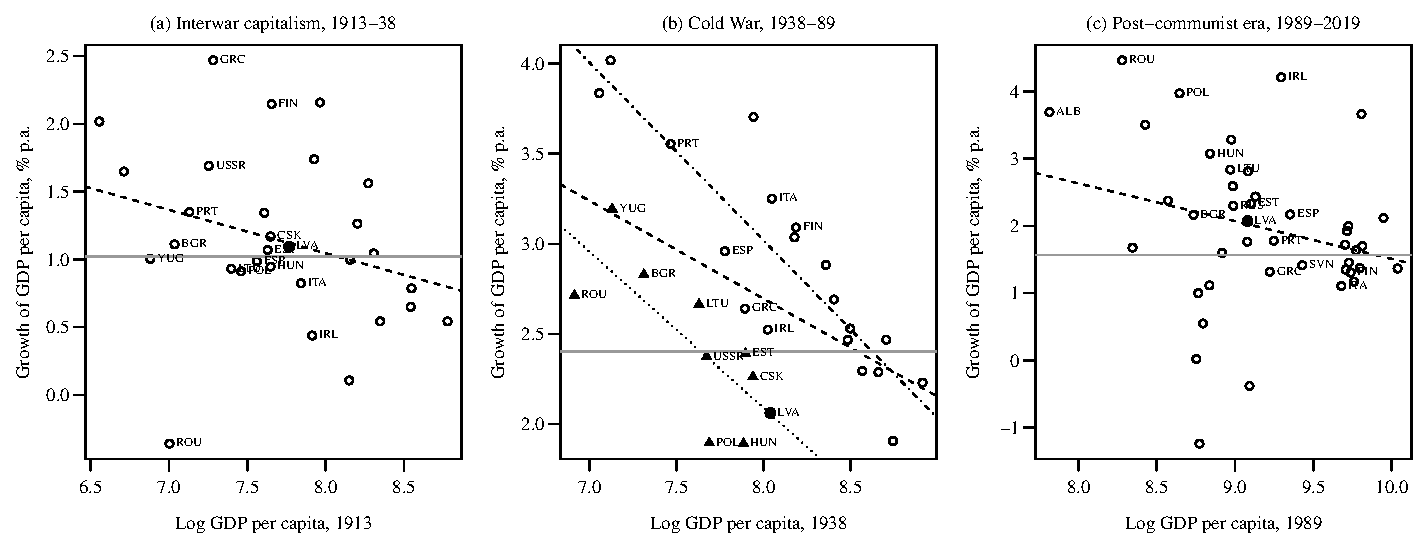
\includegraphics[width=\textwidth]{F3_beta.pdf}
\begin{minipage}{0.95\textwidth}\footnotesize
\textit{Notes:} each point is a European economy; Latvia is the filled circle and triangles in panel (b) mark the socialist economies. The dashed line is fitted to all countries, and in panel (b) the dotted line to the socialist and the dash-dotted line to the capitalist group; the grey horizontal line is the growth rate of the Western core. Spain enters panels (a) and (b) with 1935 in place of 1938 because of the civil war; Germany is omitted from panel (b). One point per economy: before 1989 the Soviet Union, Yugoslavia and Czechoslovakia enter and their member or successor states do not, except the three Baltic states; from 1989 the successor states enter and the aggregates do not. Slopes (standard errors, number of economies): (a) \betaINTERWAR{} (\betaINTERWARse{}, \betaINTERWARn{}); (b) \betaCOLDWAR{} (\betaCOLDWARse{}, \betaCOLDWARn{}); (c) \betaMODERN{} (\betaMODERNse{}, \betaMODERNn{}). Residuals of the Baltic economies from the all-country line, percentage points a year: (a) Latvia \bresINTERWARLatvia{}, Lithuania \bresINTERWARLithuania{}, Estonia \bresINTERWAREstonia{}; (b) \bresCOLDWARLatvia{}, \bresCOLDWARLithuania{}, \bresCOLDWAREstonia{}; (c) \bresMODERNLatvia{}, \bresMODERNLithuania{}, \bresMODERNEstonia{}; the residual standard deviations are \betaINTERWARsigma{}, \betaCOLDWARsigma{} and \betaMODERNsigma{}. \intlnineteen{}. \textit{Sources:} this paper, the companion series and \textcite{mpd2023}.
\end{minipage}
\end{figure}

In the interwar panel the fitted line slopes gently downward, by \betaINTERWAR{} percentage points of annual growth for each unit of log initial income, and most of the poor countries that lie below it are the East-Central European economies, including the Baltic states, that would later adopt state socialism; Latvia and Estonia lie close to the line and above Western-core growth, Lithuania well below it. The Cold War panel shows two regimes rather than one. Among capitalist economies convergence was pronounced, and every member of the Western periphery outgrew the core; among socialist economies the fitted line lies below the capitalist one at every level of income. Four of the ten, the poorest, Lithuania, Bulgaria, Yugoslavia and Romania, outgrew the Western core's \grx{Western}{1938}{1989} per cent a year; Estonia and the Soviet Union matched it; and the remaining four, Latvia among them, fell short. Latvia and Estonia nevertheless lie above the socialist line and so were among the better performers of their group. The post-communist panel restores a single downward-sloping line, of \betaMODERN{}, and almost every peripheral economy outgrew the core; Lithuania lies well above the line, Estonia above it and Latvia on it, behind Poland, Romania, Albania and Hungary, the frontrunners of the current convergence. The regressions are descriptive, not causal. The samples are small and the slopes imprecise (the figure note gives standard errors); measurement error in initial income, of the size the margins of Section~\ref{sec:method} imply, biases the slope towards zero and moves individual residuals; and panel (b), which starts in 1938 for economies that became socialist only in 1945--8, confounds the regime with war losses that ranged from a tenth to two-thirds of income per head (Table~\ref{tab:war}), so that the framework cannot establish a causal effect of communist rule \parencite{klimantas2025thesis}. Read with those limits, the conclusion is threefold. Under neither interwar capitalism nor Soviet socialism did any Baltic economy exceed the convergence expectation set by the European pool; under socialism all three fell below it, Latvia furthest, as did every socialist economy except Yugoslavia; and under restored capitalism Lithuania has exceeded the expectation, Estonia has exceeded it by less, and Latvia has merely met it.

\subsection{Sources of catch-up and decline}

The lack of consistent input data precludes growth accounting, but the series permit a reading of the three episodes of catch-up, the 1930s, the 1950s and 1960s and the years since 1995, and of the two reversals that separated them. The interwar catch-up was the closest the region came to Gerschenkronian automaticity: the Baltic economies were among the least industrialised in Europe, so that the industrial growth of the 1930s came from a low base and from the imitation of simple technologies, Danish cattle and Western electronics; capital was so scarce that modest investment yielded large returns; and structural backwardness insulated them from a Depression that struck the industrial economies hardest. But the episode was also conditioned. Governments mobilised savings for targeted investment; the land reforms had produced unusually egalitarian societies in which status was earned rather than inherited, the `social, political and cultural victory' of the modernisers that Rostow placed at the start of sustained growth \parencite[7]{rostow1959}; and literacy and Western legal traditions, strongest in Latvia and Estonia, eased the absorption of borrowed technology. The autarkic environment of the 1930s set the limit: whether these advantages could have been converted into sustained convergence in the open post-war order is the counterfactual that history did not run.

The socialist catch-up of 1950--68 was driven by the four automatic mechanisms at once, technology transferred from an already industrialised Union, capital deepening from a low base, labour moved off the land, and scale economies within a vast internal market, and it was enabled by two conditions: the social capability inherited from the interwar years, which made Latvia and Estonia, with their skilled workforces and intact infrastructure, the natural recipients of Soviet mass-production technology; and the coercion of a system that could collectivise agriculture, direct labour and investment across borders without friction, and import workers by the hundred thousand. The reversal after 1968 reflects the exhaustion of those conditions and the character of the system. By the 1970s mechanisation and industrialisation in the Baltic republics had reached Soviet levels, the labour reserve of the northern republics was spent, investment was redirected, and the educational lead that had distinguished Latvia and Estonia within the Union had eroded. What remained was the Soviet institutional system itself, which, as Crafts and Toniolo argue for the Union as a whole, could neither price resources rationally, nor reward innovation, nor move from mass production to flexible production and the service economy that were transforming the capitalist periphery across the Gulf of Finland \parencite[314--15, 323]{craftstoniolo2010}; and, as Vonyó and Klein have shown for East-Central Europe, it also failed to sustain the capital formation its own statistics claimed \parencite{vonyo_whydidsocialistfail}. Having converged on the rest of the Union in social capability and probably in capital stock, and having no control over policy, the Baltic republics most likely shared in the collapse of the Soviet growth model for the reasons that apply to the Union as a whole; that Latvia, which had converged furthest and had the heaviest concentration of all-Union industry, stagnated first is consistent with that reading, but the republic-specific policies of Moscow remain to be analysed before it can be shown to follow from it.

The modern catch-up has again drawn on the advantages of backwardness, in the form of the structural distortions and obsolete capital the Soviet era left behind, cheap and educated labour and the opening of capital and trade flows; but it has been more plainly conditional than either of its predecessors, resting on the reforms of the 1990s and the discipline of EU accession, and it has been uneven in a way that the automatic mechanisms cannot explain. Latvia, which in 1938 had the strongest prerequisites of the three for Western convergence, has gained least from the regime that rewards them most, and is now, by a narrow margin, the poorest. The Baltic century thus underscores the proposition with which the catch-up literature has ended: the benefits of backwardness are realised only through institutions that enhance social capability, and they can be forfeited, as Latvia's trajectory from the richest Baltic economy in 1913 to the poorest in 2024 shows, by regimes that destroy its institutional component and by policies that fail to rebuild it.
